
In this section, we begin with structures for representing strings
(Section~\ref{sec:prelim.string}), and then extend them to ARs using
graphs and matrices (Section~\ref{sec:prelim.ar}). Central to BUFIA is
Model Theory \citep{enderton2001mathematical}, which views structures
as mathematical objects, and uses formal logic to represent structural
units and the relationships between them. Model-theoretic analysis has
been used to compare differences between different representational
theories of phonological structure
\citep{strother2017using
	oakdenNotationalEquivalenceTonal2020, jardineetal20qtheoryAP}.  
The matrix-based representation used here is a common method in
mathematics and a particularly convenient way to represent AR
graphs. These formal representations are essential for subsequent 
algorithm development and for understanding the properties and 
learnability of ARs.

\subsection{String Representations}\label{sec:prelim.string}
Tonal melodies can be represented as strings, that is, sequences of
symbols.  Let $\Sigma$ be a finite alphabet of symbols and $\Sigma^*$
the set of all strings over $\Sigma$. For example, in a language with
a tonal inventory $\{H, L\}$, we have $\Sigma = \{H, L\}$, and
$\Sigma^*$ contains all possible strings over $\Sigma$, such as
\textit{HL}, \textit{HHL}, \textit{HLHL}, and so on. Let $|w|$ 
denote the length of a string $w$. For $0 \le n < m \le |w|$,
let $w[n:m]$ denote a non-empty substring of $w$
starting at position $n$ and ending just before position $m$.
The empty string $\epsilon$ is trivially a substring of every string.

A string can also be represented \textit{model-theoretically} with two
components: the domain $D$ and a finite set of $n$-ary relations
$\mathcal{R} = \{ R_1, R_2, \ldots, R_i \}$ \citep{rogers2013,
	chandleeBufia2019, rogers.lambert2019mol}.  A string model of
\textit{HLHL} is shown in Figure~\ref{fig.model.str}.  In this
model, $D = \{1, 2, 3, 4\}$ indicates that there are four elements in
the string. Positions $\{1, 3\}$ are 
labelled with the unary relation $H$, while $\{2, 4\}$ are the
positions labelled with $L$.  Elements are connected via a
binary \textit{successor} relation, denoted by $\lhd$.  For example,
$\lhd = \{\langle 1, 2\rangle, \langle 2, 3\rangle, \langle 3,
4\rangle\}$ specifies that position 1 (labelled $H$) immediately
precedes position 2 (labelled $L$), and position 2 immediately precedes
position 3, and so on.


\chapter{Formal Background} 
\label{chap:formal}
As discussed in Chapter~\ref{chap:tones}, tonal forms across languages have been 
analyzed using a variety of notations and representations. One question addressed 
in this dissertation is how these competing theories and representations can be 
compared systematically within a unified formal framework. Establishing such a 
framework allows us to determine how the representations differ and how structural
differences induce different generalizations about languages.

In this dissertation, I adopt a model-theoretic framework 
\citep{enderton2001mathematical,strother2017using,jardine16dissertation} to formalize 
different phonologicals representations as mathematical objects. More specifically, 
each phonological representation is modeled as a relational structure \citep{rogers.lambert2019mol}. 
The representations differ in the elements included in their domains, the relations defined 
among those elements, as well as the linguistic interpretations (or labels) assigned to 
those relations. As the following sections demonstrate, this abstraction allows competing 
representations to be expressed within a shared mathematical vocabulary without eliminating 
the structural distinctions among them. It therefore provides a principled basis for comparing 
expresivity and complexities of various representations.

This chapter organizes as follows. Section~\ref{sec:prelim} establishes the basic terminologies
in Model Theory, where we starts from the simplest representation \textit{string}, then move on 
to feature bundles, then finally multi-tiered representations and the dervied representations
couched in it.

\section{Preliminaries} \label{sec:prelim} 

\subsection{Relation, Model}

A model is a mathematical object or, in the terminology of \citet{rogers.lambert2019mol}, a \emph{relational structure}. 
A phonological representation can therefore be formalized as a model.

A model \(\mathcal{M}\) consists of a domain together with a collection of relations:

$
\mathcal{M}
\left\langle
D, (R_i)_{i \in I}
\right\rangle.
$


Here, \(\mathcal{M}\) is a model, D is a nonempty domain containing the elements of the representation, and \((R_i)_{i\in I}\) 
is an indexed family of relations defined over those elements. In a finite phonological representation, the elements of \(D\) may be indexed using natural numbers, but the domain itself consists of phonological objects, such as tones, segments, syllables, or moras.

A relation may be unary. A unary relation identifies a property or category of an individual element. For example, \(p(x)\)
means that the element x has the property of being p. In a tonal representation, \(H(x)\) means that \(x\) is an element of the domain with the property of being a high tone. Formally, a unary relation is a subset of the domain:

A relation may also be binary. A binary relation specifies a connection between two elements.
Commonly seen binary relations in phonology are include in Table~\ref{tab:binary-relations}.

\begin{table}[htbp]
    \centering
    \begin{tabular}{lll}
        \toprule
        \textbf{Binary relation} & \textbf{Notation} & \textbf{Interpretation} \\
        \midrule
        Successor   & $\lhd(x,y)$            & $x$ immediately precedes $y$ \\
        Precedence  & $<(x,y)$                & $x$ precedes $y$ \\
        Dominance   & $\operatorname{dom}(x,y)$ & $x$ dominates $y$ \\
        Association & $\alpha(x,y)$          & $x$ is associated to $y$ \\
        \bottomrule
    \end{tabular}
    \caption{Binary relations used in phonological representations}
    \label{tab:binary-relations}
\end{table}



Different phonological representations can therefore be compared by examining the elements included in their domains and the relations defined over those elements.


In this section, we begin with structures for representing strings
(Section~\ref{sec:prelim.string}), and then extend them to ARs using
graphs and matrices (Section~\ref{sec:prelim.ar}). Central to BUFIA is
Model Theory \citep{enderton2001mathematical}, which views structures
as mathematical objects, and uses formal logic to represent structural
units and the relationships between them. Model-theoretic analysis has
been used to compare differences between different representational
theories of phonological structure
\citep{strother2017using
	oakdenNotationalEquivalenceTonal2020, jardineetal20qtheoryAP}.  
The matrix-based representation used here is a common method in
mathematics and a particularly convenient way to represent AR
graphs. These formal representations are essential for subsequent 
algorithm development and for understanding the properties and 
learnability of ARs.

\subsection{String Representations}\label{sec:prelim.string}
Tonal melodies can be represented as strings, that is, sequences of
symbols.  Let $\Sigma$ be a finite alphabet of symbols and $\Sigma^*$
the set of all strings over $\Sigma$. For example, in a language with
a tonal inventory $\{H, L\}$, we have $\Sigma = \{H, L\}$, and
$\Sigma^*$ contains all possible strings over $\Sigma$, such as
\textit{HL}, \textit{HHL}, \textit{HLHL}, and so on. Let $|w|$ 
denote the length of a string $w$. For $0 \le n < m \le |w|$,
let $w[n:m]$ denote a non-empty substring of $w$
starting at position $n$ and ending just before position $m$.
The empty string $\epsilon$ is trivially a substring of every string.

A string can also be represented \textit{model-theoretically} with two
components: the domain $D$ and a finite set of $n$-ary relations
$\mathcal{R} = \{ R_1, R_2, \ldots, R_i \}$ \citep{rogers2013,
	chandleeBufia2019, rogers.lambert2019mol}.  A string model of
\textit{HLHL} is shown in Figure~\ref{fig.model.str}.  In this
model, $D = \{1, 2, 3, 4\}$ indicates that there are four elements in
the string. Positions $\{1, 3\}$ are 
labelled with the unary relation $H$, while $\{2, 4\}$ are the
positions labelled with $L$.  Elements are connected via a
binary \textit{successor} relation, denoted by $\lhd$.  For example,
$\lhd = \{\langle 1, 2\rangle, \langle 2, 3\rangle, \langle 3,
4\rangle\}$ specifies that position 1 (labelled $H$) immediately
precedes position 2 (labelled $L$), and position 2 immediately precedes
position 3, and so on.

\begin{figure}
	\centering	
	\begin{minipage}[r]{0.4\textwidth}
		\centering
		\begin{tikzpicture}[
			scale=.5,
			node distance=1.5cm,
			state/.style={draw,circle,minimum size=0.6cm}
			]
			\node[state] (1) {1\textsubscript{H}};
			\node[state,right of=1] (2) {2\textsubscript{L}};
			\node[state,right of=2] (3) {3\textsubscript{H}};
			\node[state,right of=3] (4) {4\textsubscript{L}};
			
			\draw (1) -- (2) node[midway, above]  {$\lhd$};
			\draw (2) -- (3) node[midway, above]  {$\lhd$};
			\draw (3) -- (4) node[midway, above]  {$\lhd$};

		\end{tikzpicture}
	\end{minipage}
	\hfil
	\begin{minipage}[l]{0.40\textwidth}
		\small
		\[
		\begin{aligned}
			\mathcal{M} &= \{D \mid H,L,\lhd\} \\
			D           &= \{1,2,3,4\} \\
			H           &= \{1,3\} \\
			L           &= \{2,4\} \\
			\lhd        &= \{\langle1,2\rangle,\langle2,3\rangle,\langle3,4\rangle\}
		\end{aligned}
		\]
	\end{minipage}
	\caption{String model for \textit{HLHL} over $\Sigma=\{H,L\}$.}
	\label{fig.model.str}
\end{figure}

\subsection{Feature Representations}\label{sec:prelim.feature}

\subsection{Autosegmental Representation as Graphs}\label{sec:prelim.ar}

Unlike the string model, where elements are ordered linearly along a
single axis, an AR distributes linguistic information
across multiple tiers. In this work, in addition to the basic tone and
syllable tiers, we incorporate a mora tier, 
and treat the mora as a secondary unit subordinated
to syllables to indicate the syllable weight. Therefore,
we assume each syllable must be associated with at least one
mora. %, with a pre-specified association line connecting them.
Figure~\ref{fig.model.AR1} illustrates a disyllabic form with an
LH.H melody, which is visualised as a graph in 
Figure~\ref{fig.model.AR2}, which corresponds to the model-theoretic 
relational structure in Figure~\ref{fig.model.AR3}.


\begin{figure}[ht]
	\centering
	% Autosegmental Representation
	\begin{minipage}[b]{0.2\textwidth}
		\centering
		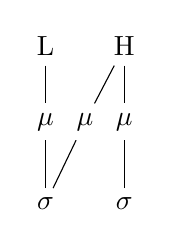
\begin{tikzpicture}
			\node (t1) at (1,1) {L};
			\node (t2) at (2,1) {H};
			
			\node[anchor=base] (c1) at (1,0) {$\mu$};
			\node[anchor=base] (c2) at (1.5,0) {$\mu$};
			\node[anchor=base] (c3) at (2,0) {$\mu$};
			
			\node (s1) at (1,-1) {$\sigma$};
			\node (s2) at (2,-1) {$\sigma$};
			
			\draw (t1) -- (c1);
			\draw (t2) -- (c2);
			\draw (t2) -- (c3);
			\draw (s1) -- (c1);
			\draw (s1) -- (c2);
			\draw (s2) -- (c3);            
		\end{tikzpicture} \vspace{2em}
		\subcaption{AR}
		
		\label{fig.model.AR1}
	\end{minipage}
	\hfill
	% Graph Representation
	\begin{minipage}[b]{0.4\textwidth}
		\centering
		\begin{tikzpicture}[scale=0.5]
			\node[state] (t1) at (0,6) {1\textsubscript{L}};
			\node[state] (t2) at (6,6) {2\textsubscript{H}};
			
			\node[state] (c1) at (0,3) {3\textsubscript{$\mu$}};
			\node[state] (c2) at (3,3) {4\textsubscript{$\mu$}};
			\node[state] (c3) at (6,3) {5\textsubscript{$\mu$}};
			
			\node[state] (s1) at (0,0) {6\textsubscript{$\sigma$}};
			\node[state] (s2) at (6,0) {7\textsubscript{$\sigma$}};
			
			\draw (t1) -- node[midway, left]   {$\alpha$} (c1) -- node[midway, left]
			{$\alpha$}(s1);
			\draw (t2) -- node[midway, left] {$\alpha$} (c2) -- node[midway, left]
			{$\alpha$}(s1);
			\draw (t2) -- node[midway, right] {$\alpha$} (c3) -- node[midway, right]
			{$\alpha$}(s2);
			
			
			\draw (t1) -- node[midway, above]  {$\lhd$} (t2);
			\draw (c1) -- node[midway, above]  {$\lhd$}(c2);
			\draw (c2) -- node[midway, above]  {$\lhd$}(c3);
			\draw (s1) -- node[midway, above]  {$\lhd$}(s2);
		\end{tikzpicture}
		\subcaption{Graph}
		\label{fig.model.AR2}
	\end{minipage}
	\hfill
	% Model Representation
	\begin{minipage}[b]{0.3\textwidth}
		\small
		\centering
		\begin{align*}
			%            M &= \langle D|  H, L, \mu, \sigma, \lhd, \alpha \rangle \\
			D &= \{1, 2, 3, 4, 5, 6, 7\} \\
			L &= \{1\}\\
			H &= \{2\}\\
			\mu &= \{3, 4, 5\}\\
			\sigma &= \{6, 7\} \\
			\lhd &= \{\, \langle 1,2 \rangle, \langle 3,4 \rangle, \langle 4,5 \rangle,
			\langle 6,7 \rangle\} \\
		\alpha &= \left\{
		\begin{aligned}
			&(1,3),(2,4),(2,5),\\
			&(3,6),(4,6),(5,7)
		\end{aligned}
		\right\}
		\end{align*}
		\subcaption{Model}
		\label{fig.model.AR3}
	\end{minipage}
	
	
	\caption{Three representations of a disyllabic LH.H}
	\label{fig.model.AR}
\end{figure}

A graph consists of a set of vertices $V$ and edges $E$.  
As shown in Figure~\ref{fig.model.AR3}, the graph consists
of seven \textit{labelled nodes} which are circles numbered with $\{1, 2,\dots,7\}$, 
representing linguistic units, each labelled with its corresponding properties, such
as $L$, $H$, $\sigma$, or $\mu$. 
The lines connecting elements are referred to as \textit{edges}, which 
may be either \textit{directed} or \textit{undirected}. For clarity, 
we distinguish two types of connections: \textit{association relations}, 
denoted by $\alpha$, refer to the undirected edges across tiers; 
%(e.g., between tones and moras, or between moras and syllables), 
and successor relations, denoted by $\lhd$, represent ordered relationships within a single tier. 
All the successor connections in the current example are given by
\( \lhd = \{\langle 1,2 \rangle,\ \langle 3,4 \rangle,\ \langle 4,5
\rangle,\ \langle 6,7 \rangle \}.\) The association relations, on the
other hand, are expressed as a set of unordered pairs:
\(\alpha = \{ (1,3),\ (2,4),\ (2,5),\ (3,6),\ (4,6),\ (5,7) \}.\)
Together, the tuple $\langle H, L, \mu, \sigma, \lhd, \alpha \rangle$
constitutes the \textit{signature} of this model-theoretic representation
of an AR.

In addition to representing model-theoretic relational structures 
with graphs, one can use \textit{adjacency matrices}
\citep{west2001introduction,CLRS2022}, which use binary values to
denote whether there is an edge between two nodes. Two nodes, $v$ and
$w$, are considered \textit{adjacent} if there is an edge connecting
them. If $G$ is a graph with $n$ nodes %,labelled $\{1, 2, \ldots, n\}$,
then its adjacency matrix $A$ is an $n \times n$ matrix. If $i$ and 
$j$ are connected, the entry $(i, j)$ has the value of 1; otherwise it is
0. 
Using this method, an AR with $t$ tones, $m$ moras, and $s$ 
syllables can be encoded as a $t \times m$ tone-mora matrix and 
a $m \times s$ mora-syllable matrix, with successor relations 
implicit in the indexing. For instance, Table~\ref{tab.matrices} provides an alternative
representation of the same AR in Figure~\ref{fig.model.AR}.
In the tone-mora matrix, the header row reflects the tonal sequence
$LH$, and the index column reflects the mora sequence. Since the L tone is
associated with the first mora $\mu_1$, and the H tone is associated with
both $\mu_2$ and $\mu_3$, the corresponding cells
$(L, \mu_1), (H, \mu_2), (H, \mu_3)$ are marked with 1, and the others
with 0 which indicates no connection between them.\footnote{For
	convenience, we refer to each cell by the labels of the nodes. Node
	indices will be omitted from here on. For example, we may refer to $(1,3)$
	and $(2,4)$ with $(L,\mu_1)$ and $(H, \mu_2)$, respectively. However, 
	these are the labels of the nodes rather than the nodes 
	themselves.}  If we examine the matrix by columns, one can infer that
the L tone occupies the first mora, while the H tone occupies the
remaining two.  Likewise, in the mora syllable matrix, since
$\sigma_1$ is associated with $\mu_1$ and $\mu_2$, and $\sigma_2$ with
$\mu_3$, the corresponding cells are marked with 1. If we examine this
matrix by rows, it can be seen that $\sigma_1$ is heavy while
$\sigma_2$ is light. Hereafter, we refer to the rows and columns in
the tone-mora matrix as the mora rows and tone columns respectively;
and to the rows and columns in the mora-syllable matrix as the
syllable rows and mora columns respectively.
\begin{table}[ht]
\centering 
	\begin{tabular}{cc}
	\centering
	\begin{tabular}{c|cc}
			& L & H \\
			\hline
			$\mu_1$ & 1 & 0 \\
			$\mu_2$ & 0 & 1 \\
			$\mu_3$ & 0 & 1 \\
	\end{tabular} \vspace{1em}
		&
	\begin{tabular}{c|ccc}
			& $\mu_1$ & $\mu_2$ & $\mu_3$ \\ \hline
			$\sigma_1$ & 1     & 1     & 0     \\
			$\sigma_2$ & 0     & 0     & 1
	\end{tabular}
	\end{tabular}
	\caption{Adjacency matrices: tone–mora matrix (left) and mora–syllable matrix (right)}
	
	\label{tab.matrices}
\end{table}

These AR adjacency matrices capture precisely the same information as
the graphs and model-theoretic structures. If we replace the header
row and index column with the node numbers used in the graph model
signature, and replace the 1s with the indices of row and column, we
obtain the table filled as in Table~\ref{tab.index}. As can be
seen, these pairs are identical to the information encoded in
Figure~\ref{tab.matrices}.

\begin{table}[ht]
	\centering
	\begin{tabular}{cc}
		$\begin{array}{c|c@{}c@{}c}
			& 1 & \lhd & 2 \\
			\hline
			3 & (1,3)  && 0 \\
			\lhd & && \\
			4 & 0 & & (2,4) \\
			\lhd & && \\
			5 & 0 & & (2,5) \\
		\end{array}$ \hspace{1em} &
		$\begin{array}{c|c@{}c@{}c@{}c@{}c}
			& 3 & \lhd & 4 & \lhd & 5 \\
			\hline
			6           & (3,6) &         & (4,6) &         &   	\\
			\lhd  &       &         &       &         &   	\\
			7           &       &         &       &         & (5,7) \\
		\end{array}$
	\end{tabular}
\caption{Equivalent node-indexed encodings of the adjacency matrices in Table~\ref{tab.matrices}, where $\lhd$ and $\alpha$ are the successor and association predicates of the model signature.}
	\label{tab.index}
\end{table}

Furthermore, certain patterns can be easily identified by inspecting the
matrices. For example, a series of contiguous 1s may indicate tone 
spreading over multiple moras if observed in the tone column, or a mora 
shared by multiple tones if seen in the mora row. 
Two 1s positioned diagonally suggest a one-to-one mapping.
The associations $(L,\mu_1)$ and $(H,\mu_2)$
in the tone-mora matrix in Table \ref{tab.matrices}
present an example of this.
Some particular or ill-formed patterns can also be 
readily detected, which will be discussed in Section~\ref{sec:bufiaar}.


\subsection{Structure Containment}
%
An important concept when considering model-theoretic relational
structures, either strings, sequences of feature bundles, or ARs, is
\textit{containment}. Intuitively, containment refers to the situation
when one structure includes another structure inside of it. We
formalise this notion using two related definitions, following
\citet{chandleeBufia2019}: \textit{restriction}
(Definition~\ref{def.res}) and \textit{containment}
(Definition~\ref{def.contain}). Readers are referred to
\citet{rogers.lambert2019mol} for an alternative formulation. In the
definitions below, it is assumed the structures A and B have the same
signature $\langle R_1, \ldots R_n \rangle$.

\begin{definition}
	\label{def.res}
	\textit{ $A= \langle D^A; R^A_1, \ldots, R^A_n \rangle$ is a \emph{restriction}
		of $B
		= \langle D^B; R^B_1, \ldots, R^B_n \rangle$ iff $D^A \subseteq D^B$ and for
		each $m$-ary relation $R^A_i$, we have $R^A_i = \{(x_1, \ldots, x_m) \in R^B_i \mid x_1, \ldots, x_m \in D^A\}$. }
\end{definition}

\begin{definition}
	\label{def.contain}
	\textit{Structure $A$ is \emph{contained} in structure $B$
		($A \sqsubseteq B$) if there exists a restriction of $B$, denoted
		$B'$, and there exists a function $h:A \rightarrow B'$ such that for
		each $m$-ary relation $R_i$ in the model signature:
		\(R_i(a_1, \ldots, a_m) \in A \implies R(h(a_1), \ldots, h(a_m)) \in
		B'.\)}
\end{definition}

These definitions mean that $A$ is \textit{contained} in $B$ whenever
there exists a subpart of $B$ onto which \(A\) projects via a function
\(h\), and furthermore, that the relations that hold among elements of
\(A\) hold among their corresponding elements in \(B\). For instance,
the AR in Figure~\ref{fig.restriction:a} is contained in the AR
in Figure~\ref{fig.restriction:b} because the dotted region in
\ref{fig.restriction:b} preserves all internal relations of
%:
\ref{fig.restriction:a}, despite the differences in the
indexing. In particular, $\mu_1, \mu_2, \sigma_1$ in
\ref{fig.restriction:a} project to $\mu_2, \mu_3, \sigma_2$ in
\ref{fig.restriction:b}, respectively.


\begin{figure}[h]
	\centering
	\begin{minipage}[t]{0.32\textwidth}
		
		
		\centering
		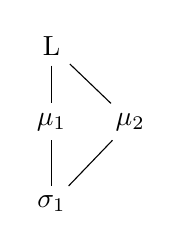
\begin{tikzpicture}
			\node (t2) at (1,1) {L};
			
			\node[anchor=base] (c1) at (1,0) {$\mu_1$};
			\node[anchor=base] (c2) at (2,0) {$\mu_2$};
			
			\node (s2) at (1,-1) {$\sigma_1$};
			\draw (t2) -- (c1) -- (s2);
			\draw (t2) -- (c2) -- (s2);
			
		\end{tikzpicture} 
		\subcaption{Heavy L syllable}
		\label{fig.restriction:a}
	\end{minipage}	
	\begin{minipage}[t]{0.32\textwidth}
		\begin{tikzpicture}
			\node (t1) at (1,1) {H};
			\node (t2) at (2,1) {L};
			\node (t3) at (3,1) {H};
			
			\node[anchor=base] (c1) at (1,0) {$\mu_1$};
			\node[thick, anchor=base] (c2) at (2,0) {$\mu_2$};
			\node[thick, anchor=base] (c3) at (3,0) {$\mu_3$};
			
			\node (s1) at (1,-1) {$\sigma_1$};			
			\node (s2) at (2,-1)  {$\sigma_2$};
			\draw (t1) -- (c1) -- (s1);
			\draw (t2) -- (c1) -- (s1);
			\draw (t2) -- (c3) --(s2);
			\draw  (t2) -- (c2) -- (s2);
			\draw  (t3) -- (c3);
			\draw[dotted, thick]
			($(t2)+(-0.3,0.3)$) --
			($(t2)+(0.2,0.3)$) --
			($(c3)+(0.3,0.2)$) --
			($(c3)+ (0.3,0.2) + (0,-0.45)$) --
			($(s2)+(0.2,-0.3)$) --
			($(s2)+(-0.3,-0.3)$) --
			cycle;
			
			
		\end{tikzpicture} 
		\subcaption{AR containing a heavy L}
		\label{fig.restriction:b}
	\end{minipage}
	\caption{A heavy L-toned syllable and a structure in which it is contained}
	\label{fig.restriction}
\end{figure}


The containment relation is particularly important because it provides
a natural \textit{ordering} over the space of possible structures. The
ordering is not total, like a linear order; it is a \textit{partial}
ordering. In such a partially-ordered space, some structures are
comparable in terms of containment, but not necessarily all of them
are. \citet{chandleeBufia2019} provides some additional terminology:
if one structure \(A\) is contained in another structure \(B\), then
structure \(A\) is a \textit{subfactor} of structure \(B\), whereas
\(B\) is a \textit{superfactor} of \(A\). They prefer these terms to
substructures and superstructures, which have different
technical meanings in model theory.

To illustrate, Figure~\ref{fig.hasse.str} displays a
non-exhaustive portion of the partial ordering of possible strings
over the alphabet $\Sigma = \{a,b\}$. At the bottom of the ordering is
the empty string $\epsilon$, with more complex strings appearing
higher in the ordering.  Whenever two elements are connected by a
line, it means that the higher element contains the lower element. For
example, no line relates the \(a\) to \(b\), because neither contains
the other.  However, a line is drawn from \(a\) to \(aa, ab\) and
\(ba\), because \(a\) is contained in each of these structures. As
defined above, \(aa, ab, ba\) and \(aaa\), and any other strings that
contain \(a\) are superfactors of \(a\); correspondingly, \(a\) is a
subfactor of each of these strings.

There can be many layers between a superfactor and one of its 
subfactors. When there are no structures ordered 
between a superfactor and one of its subfactors, the 
superfactor is called a \textit{next superfactor}. 
In this sense, among all superfactors of \(a\) such as 
\(\{aa, ab, ba, aaa, aab, \cdots\}\), only those superfactors that 
are exactly one level above are next superfactors of \(a\), 
namely \(\{aa, ab, ba\}\).

\begin{figure}
	\centering
	\begin{tikzpicture}[
		every node/.style={inner sep=1pt, font=\small\itshape},
		edge/.style={},
		]
		\matrix (m) [matrix of nodes,
		row sep=6mm,
		column sep=10mm,
		nodes={anchor=center},
		]{
			\node (aaa) {aaa}; &\node (llb1) {...};&   \node (llb2) {...}; & \node (llb3) {...};&\node (llb4) {...};&\node (llb5) {...};&    \node (bbb) {bbb}; \\
			&\node (aa) {aa}; & \node (ab) {ab}; && \node (ba) {ba}; & \node (bb) {bb}; \\
			&& \node (a) {a}; & & \node (b) {b}; &  \\
			&&& \node (z) {$\epsilon$}; && \\};
		
		\draw[edge] (z) -- (a);
		
		\draw[edge] (z) -- (b);
		
		\draw[edge] (a) -- (aa) -- (aaa);
		\draw[edge] (a) -- (ab);
		\draw[edge] (a) -- (ba);
		
		\draw[edge] (b) -- (bb) -- (bbb);
		\draw[edge] (b) -- (ab);
		\draw[edge] (b) -- (ba);
		\draw[edge, dotted] (aa) -- ++(0,1.5em);
		%	\draw[edge, dotted] (aa) -- ++(1,1.5em);
		\draw[edge, dotted] (ab) -- ++(0,1.5em);
		%	\draw[edge, dotted] (ab) -- ++(1,1.5em);	
		%	\draw[edge, dotted] (bb) -- ++(-1,1.5em);	
		\draw[edge, dotted] (ba) -- ++(0,1.5em);
		\draw[edge, dotted] (bb) -- ++(0,1.5em);
	\end{tikzpicture}
	\caption{Strings over $\Sigma = \{a,b\}$ ordered by the containment relation (non-exhaustive)}
	\label{fig.hasse.str}
\end{figure}%



\subsection{BUFIA}\label{sec:prelim.bufia}

Recall that given a set of positive examples, BUFIA returns a grammar just like
the ones considered by \citet{jardine2017LocalNature}: a conjunction
of negative literals: $\lnot C_1 \land \lnot C_2 \land \ldots \land \lnot C_n$.
BUFIA begins its search of the possible structure space with the most
general structure (the empty structure) and progresses to more
specific ones. In other words, it proceeds from the bottom of the
inverted pyramid upwards. In this process, two functions are central 
to BUFIA: \textsc{Contain} and \textsc{NextSupFact}. For each 
candidate structure \(S\), BUFIA applies the
\textsc{Contain} function to check whether it is attested
in the positive data. If it is, BUFIA concludes it is not a bona-fide
constraint, discards it, and uses \textsc{NextSupFact} to generate a
set of next superfactors to continue the search. If, on the other
hand, \(S\) is absent from the positive data, it is added to the
grammar as a constraint. For structures that are labelled as constraints,
BUFIA does not apply \textsc{NextSupFact}. Consequently, all structures/possible 
constraints that contain it are pruned from the remaining search. The learning 
process continues until a stopping condition is met, which in this work is a
predetermined upper bound on the size of the constraints.

Using the same example from Figure~\ref{fig.hasse.str}, suppose
the language forbids adjacent \(b\)s, formalised as a constraint
\(^*bb\), which excludes strings \(\{bb, bba, bbb, abb,
\cdots\}\). For concreteness, assume a data set \(D = 
\{aba, baabaa\}\).  BUFIA begins from the most general hypothesis:
applies \textsc{Contain} to check whether the empty string $\epsilon$
is attested in the positive data.  Since $\epsilon$ is contained in
every string trivially, \textsc{Contain} returns true, and BUFIA does
not add $\epsilon$ as a constraint. Then, BUFIA applies
\textsc{NextSupFact} to generate the next superfactors of $\epsilon$,
which are the two singletons \(a\) and \(b\). In a breadth-first
order, BUFIA checks whether \(a\) and \(b\) are contained in the
positive data.  In the same fashion, the \textsc{Contain} function
confirms both strings are attested as substrings of \(D\), discards
them, and then generates their superfactors for later checking. When
BUFIA reaches \(bb\), \textsc{Contain} returns false because
\(bb\) is not contained in any datum in the data set (neither \(aba\) nor 
\(baabaa\) contains \(bb\)). BUFIA therefore adds
\(^*bb\) to the grammar and skips generating any superfactors of
\(bb\). The search then continues with the remaining candidates until
the stopping condition is met (e.g., the size of structures exceeds a
predefined size such as two).\footnote{An alternative stopping
  condition is to set a number of constraints. Both kinds of stopping
  conditions control the amount of generalisation. The longer the
  search is permitted, more constraints may be found, and amount of
  generalisation is reduced. Without any limits, it will overfit the
  data. However, when the search terminates sooner, generally fewer
  constraints will be found, and the grammar makes broader
  generalisations.}

\citet{chandleeBufia2019} prove that BUFIA returns a set of
constraints that (1) are consistent with the data (no constraint
returned by BUFIA is contained in any datum in the positive data); (2)
contain the most general constraints (obtains the simplest possible
constraints according to the order imposed by the containment
relation, e.g.  only \(^*bb\) is returned but not \(^*bba\), \(^*bbb\)
or others); and (3) generate the smallest set of structures consistent
with the data, among the other possible grammars that are
consistent with the data subject to the same conditions (generalises
conservatively).

One concern for BUFIA is its time complexity: BUFIA runs in exponential time in the worst 
case \citep{chandleeBufia2019}. However, as \citet{Swanson+2025} 
point out, data sparsity is highly advantageous for learning since 
the hypothesis space is thus pruned more efficiently.

Another concern raised by the reviewers is that, in its
present form, BUFIA is fragile with respect to noise. For example, if
there is a single data point violating a constraint \(C\) in the
data (a ``noisy intrusion''), then \(C\) will not be included in the
output grammar, even if \(C\) is an otherwise valid
generalisation. It is important to put this current limitation in
context. First, even in the absence of noise, it is currently unknown
how to learn constraints expressed with ARs. From the viewpoint of
scientific practice, it makes sense to address an easier problem
before addressing a harder problem. Second, BUFIA can be adapted to
handle noise in different kinds of ways. Prior literature suggests
multiple strategies for handling noisy intrusions, exceptions, and
sparse data \citep{angluin88, Yang2016, Wu-Heinz-2023-SELDNI,
  Kaelbling+2023-RILIPD, Dai2025}. Considering versions of BUFIA that
are robust to all kinds of noise is a valuable direction for future
research. Third, it is worth pointing out that the mere use of
statistical methods for learning does not automatically make learners
robust to noise \citep{Angluin88b}. In other words, noisy data is an
issue, and one that can be studied separately from the fundamental
issue of successful generalisation. See \citet{Heinz2009} for
additional discussion on factoring learning problems.

\section {Transduction}

What is a transduction

string tranduction, feature transducton, AR transduction

	\begin{figure}
		\centering
		
		\begin{minipage}[t]{0.48\textwidth}
			\centering
			
			\begin{tabular}{c c c}
				
				\textbf{UR} & $\Rightarrow$ & \textbf{SR} \\[0.5em]
				
				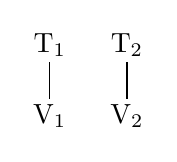
\begin{tikzpicture}[scale=0.7, every node/.style={inner sep=2pt}]
					\node (v1) at (0,0) {V$_1$};
					\node (v2) at (1.4,0) {V$_2$};
					
					\node (t1) at (0,1.3) {T$_1$};
					\node (t2) at (1.4,1.3) {T$_2$};
					
					\draw (v1)--(t1);
					\draw (v2)--(t2);
				\end{tikzpicture}
				
				&&
				
				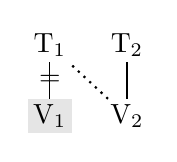
\begin{tikzpicture}[scale=0.7, every node/.style={inner sep=2pt}]
					\node [fill=gray!20](v1) at (0,0) {V$_1$};
					\node (v2) at (1.4,0) {V$_2$};
					
					\node (t1) at (0,1.3) {T$_1$};
					\node (t2) at (1.4,1.3) {T$_2$};
					
					\draw (v1)--(t1) node[midway] {=};
					\draw (v2)--(t2);
					
					\draw[dotted, thick] (v2)--(t1);
				\end{tikzpicture}
				
			\end{tabular}
			
		\end{minipage}
		\hfill
		\begin{minipage}[t]{0.48\textwidth}
			\centering
			
			\begin{tabular}{c c c}
				
				\textbf{UR} & $\Rightarrow$ & \textbf{SR} \\[0.5em]
				
				$
				\begin{array}{c|cc}
					& T_1 & T_2\\
					\hline
					V_1 & \cellcolor{gray!75}1 & 0 \\
					V_2 & \cellcolor{gray!15}0 & 1 \\
				\end{array}
				$
				
				&&
				
				$
				\begin{array}{c|cc}
					& T_1 & T_2\\
					\hline
					V_1 & \cellcolor{gray!15}0 & 0 \\
					V_2 & \cellcolor{gray!75}1 & 1 \\
				\end{array}
				$
				
			\end{tabular}
			
		\end{minipage}
		\caption{Contour formation in both graph-theoretic and matrix representations.}
		\label{fig:hiatus}
	\end{figure}
	

	

\section{Learning Algorithm}